
%(BEGIN_QUESTION)
% Copyright 2010, Tony R. Kuphaldt, released under the Creative Commons Attribution License (v 1.0)
% This means you may do almost anything with this work of mine, so long as you give me proper credit

Skisser tubeforbindelsene som trengs for å teste denne stempeldrevne reguleringsventilen på en arbeidsbenk. Anta at ventilhuset er direktevirkende, og at aktuatoren ikke har intern fjær, slik at den må testes med trykk i to retninger for først å åpne og deretter lukke ventilen. Skisser først forbindelsene som brukes for å påføre trykk og åpne ventilen:

$$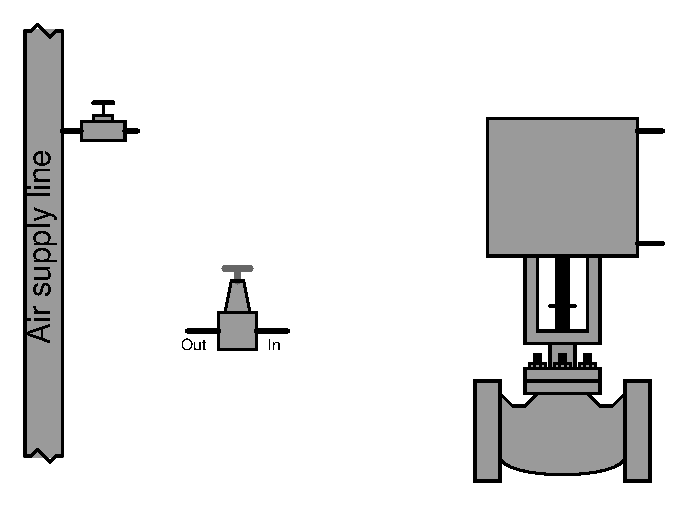
\includegraphics[width=15.5cm]{i00767x01.eps}$$

Beskriv deretter hva du ville endret for å få ventilen til å gå i lukkeretning.

\vfil

\underbar{file i00767}
\eject
%(END_QUESTION)





%(BEGIN_ANSWER)

Dette er en vurdert oppgave -- ingen svar eller hint er gitt!

%(END_ANSWER)





%(BEGIN_NOTES)

$$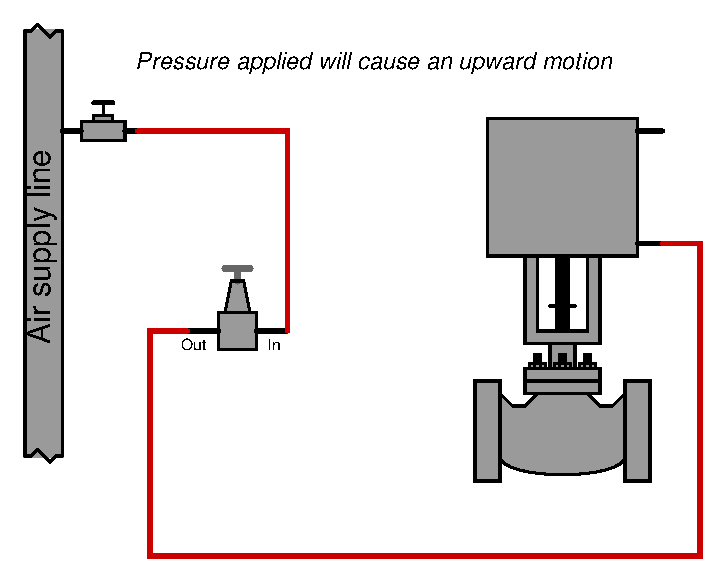
\includegraphics[width=15.5cm]{i00767x02.eps}$$

For å kjøre ventilen mot lukket posisjon flytter du regulatorens utgangsslange til øvre port på stempelaktuatoren (med avlufting av nedre port), og påfører deretter lufttrykk på nytt.

%INDEX% Sluttkontrollelementer, ventil: pneumatisk stempelaktuator

%(END_NOTES)


